\subsubsection*{Event table}
Tabellen indeholder data om events i systemet. Tabellen fungere som omdrejningspunkt i databasen. Droner, billeder og waypoints kan tilføjes til et event.
\vspace{-5pt}
\begin{figure}[H]
	\centering
	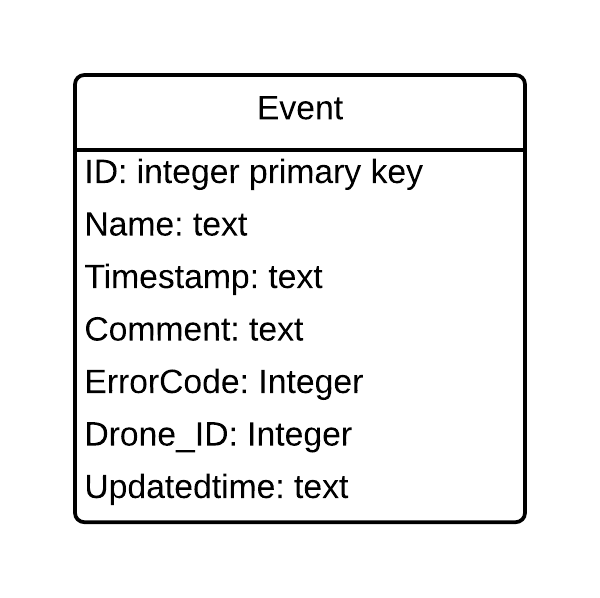
\includegraphics[width=0.5\textwidth]{Billeder/database/EventTable.png}
	\vspace{-5pt}
	\caption{Event table}
	\label{fig:event_table}
\end{figure}

\begin{table}[H]
\begin{tabular}{| p{3cm}| p{11.5cm}|}
\hline

Formål	 							& Holde data om events i systemet.\\\hline
Forbindelser						& Tabellen har en foreing key til user tabellen med en mange til mange relation. Drone-, waypoint- og picture-tabellen har foreing keys til event tabellen.\\\hline
Attributter						& \begin{itemize}
												\item ID: Primary key.
												\item Name: Navnet på det givet event. Max length: 100 char
												\item Timestamp: Timestamp for oprettelse: Datefield
												\item Updated: Timestamp for opdaterede: Datefield
												\item Comment: Kommentar til givet event. Max length: 100 char
												\item ErrorCode: Fejlkode hvis fejl opstår under flyvning: Integer
												\item UserId: Mange til mange relation til user tabellen: Foreingkey
											\end{itemize} \\\hline 
\end{tabular}
\caption{Event table}
\label{tab:event_table}
\end{table}